\subsection{Anforderungen}
Das Webinterface hat auf der einen Seite die Aufgabe die Kommunikation mit der
Kennzeichenerkennung und der Induktionmessung sicherzustellen und auf der
anderen Seite die Verwaltung und Darstellung der gewonnen Daten.

\subsection{Lokale Entwicklungsumgebung mit Laragon}
Für die Programmierung des Webinterfaces müssen zuerst einige Vorkehrungen
getroffen werden, dazu zählt zu einem die Installation von benötigter Software
und deren konfiguration.

\subsubsection{Benötigte Software}

\begin{itemize}
  \item \textbf{Laragon} (\url{https://laragon.org}) \\Beinhaltet mehrere
  Softwarepakete die für die Entwicklung notwendig sind.
  \begin{itemize}
    \item Apache HTTP Server
    \item MySQL
    \item PHP
  \end{itemize}
  \item \textbf{phpMyAdmin} (\url{https://www.phpmyadmin.net}) \\ Webinterface
  für MySQL
  \item \textbf{Composer} (\url{https://getcomposer.org}) \\ Paketmanager für
  PHP
  \item \textbf{Git} (\url{https://git-scm.com}) \\ Versionskontrolle
  \item \textbf{Visual Studio Code} (\url{https://code.visualstudio.com}) \\
  Quelltext-Editor
\end{itemize}

\subsubsection{Konfiguration von PHP}
Um PHP Befehle von der Kommandozeile auszuführen muss die Installation zuerst in
den Windows Path Variables hinzugefügt werden.

Dies erfolgt durch die \textbf{Advanced System Settings} $\blacktriangleright$
\textbf{Environment Variables} $\blacktriangleright$ \textbf{System Variables}.
Dort kann nun die Path Variable editiert werden und der Pfad hinzugefügt werden
in welchem die php.exe liegt.

\begin{figure}[H]
  \centering
  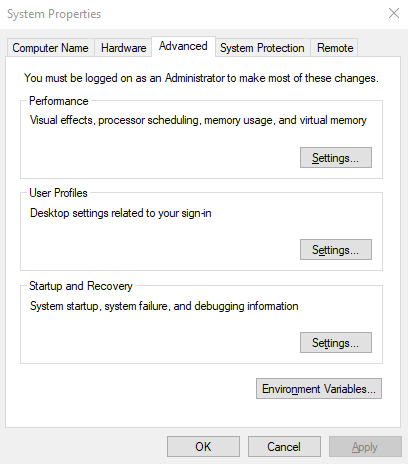
\includegraphics[width=0.6\linewidth]{webinterface/advanced_system_settings.png}
  \caption{Advanced System Settings}
\end{figure}

\begin{figure}[H]
  \centering
  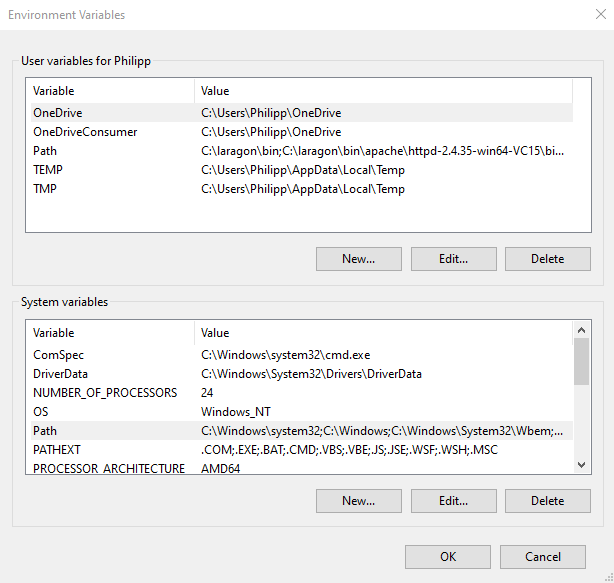
\includegraphics[width=0.6\linewidth]{webinterface/system_variables.png}
  \caption{System Variables}
\end{figure}

\begin{figure}[H]
  \centering
  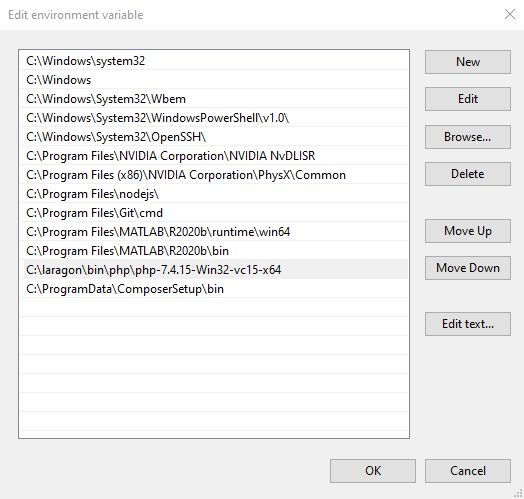
\includegraphics[width=0.6\linewidth]{webinterface/environment_variable.png}
  \caption{Environment Variables}
\end{figure}

Die korrekte konfiguration kann durch die Kommandozeile geprüft werden, dort
muss das Befehl \textbf{php -v} ausgeführt werden. Dabei ist zu beachten, dass
nach dem hinzufügen der Path Variable die gewählte Kommandozeile neu gestartet
werden muss.

\begin{figure}[H]
  \centering
  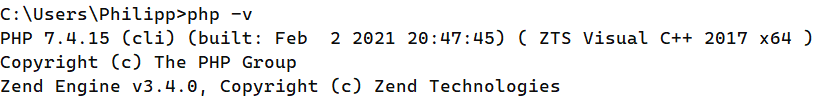
\includegraphics[width=1\linewidth]{webinterface/php_version.png}
  \caption{PHP Version}
\end{figure}

Somit ist PHP korrekt konfiguriert.

\subsubsection{Installation von phpMyAdmin}
phpMyAdmin ist ein Tool, welches den Umgang mit MySQL Datenbanken mit einem
Webinterface erleichtert. Die aktuellste Version lässt sich von
\url{https://www.phpmyadmin.net/downloads} downloaden. Dieses Archiv muss
entpackt werden und ausgehend vom Laragon Root Verzeichnis in das Verzeichnis
\textbf{/etc/apps} kopiert werden. Um die Installation zu überprüfen muss der
Apache HTTP Server und der MySQL Server gestartet werden, nun sollte bei einer
korrekten Installation das Webinterface von phpMyAdmin unter
\url{http://localhost/phpmyadmin} erreichbar sein.

\begin{figure}[H]
  \centering
  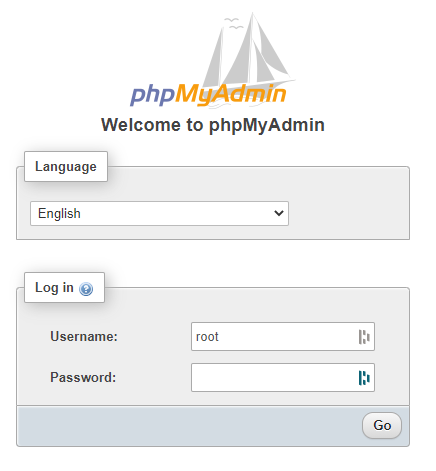
\includegraphics[width=0.5\linewidth]{webinterface/phpmyadmin.png}
  \caption{phpMyAdmin Webinterface}
\end{figure}

Es ist nicht notwendig ein Passwort einzugeben, da Standardmäßig kein Passwort
gesetzt wird.

\subsection{Lokale Entwicklungsumgebung mit WSL und Docker}

\subsubsection{Benötigte Software}

\begin{itemize}
  \item \textbf{Docker} (\url{https://www.docker.com}) \\ Ermöglicht Isolation
  von Anwendungen mit Containervirtualisierung
  \item \textbf{WSL} (\url{https://docs.microsoft.com/en-us/windows/wsl}) \\
  Kompatibilitätsschicht für Linux Anwendungen unter Windows 10
  \item \textbf{Visual Studio Code} (\url{https://code.visualstudio.com}) \\
  Quelltext-Editor
\end{itemize}

\subsubsection{Installation von WSL}
Zuerst müssen einige Einstellungen in Windows getroffen werden um später eine
Linux Distribution herunterzuladen können. Diese Befehle können über die
Kommandozeile mit Administrativen Rechten ausgeführt werden.

\paragraph{1. Schritt: WSL Aktivieren}\mbox{}\\
\begin{lstlisting}[caption={WSL Feature Feature aktivierens}, captionpos=b]
  dism.exe /online /enable-feature
  /featurename:Microsoft-Windows-Subsystem-Linux /all /norestart
\end{lstlisting}

\paragraph{2. Schritt: Virtual Machine Aktivieren}\mbox{}\\
\begin{lstlisting}[caption={Virtual Machine Feature aktivieren}, captionpos=b]
  dism.exe /online /enable-feature /featurename:VirtualMachinePlatform /all
  /norestart
\end{lstlisting}

Nach diesem Schritt ist ein Neustart des Computers notwendig.

\paragraph{3. Schritt: Linux Kernel Update}\mbox{}\\
Nun muss ein Linux Kernel Update installiert werden, die aktuelle Version ist
unter \url{https://aka.ms/wsl2kernel} zu finden.

\paragraph{4. Schritt: WSL 2}\mbox{}\\
Nach dem Neustart des Computers sollte es nun möglich sein WSL 2 als Version
auszuwählen.
\begin{lstlisting}[caption={WSL 2 auswählen}, captionpos=b]
  wsl --set-default-version 2
\end{lstlisting}

\paragraph{5. Schritt: Linux Distribution herunterladen}\mbox{}\\
Zuletzt kann eine Linux Distribution aus dem Windows Store heruntergeladen
werden, in diesem Fall Debian (\url{https://www.microsoft.com/de-de/p/debian}).

\subsubsection{Installation von Docker}
Die aktuellste Version von Docker Desktop für Windows lässt sich am einfachsten
über die offizielle Website von Docker herunterladen (\url{https://docker.com}).
Nach der Installation muss noch die WSL Integration aktiviert werden. Dazu muss
in den Einstellungen unter \textbf{Resources} $\blacktriangleright$ \textbf{WSL Integration} und
dort muss der Haken bei \textbf{Enable integration with my default WSL distro} gesetzt
werden und die installierte Linux Distribution muss unten aktiviert werden.

\begin{figure}[H]
  \centering
  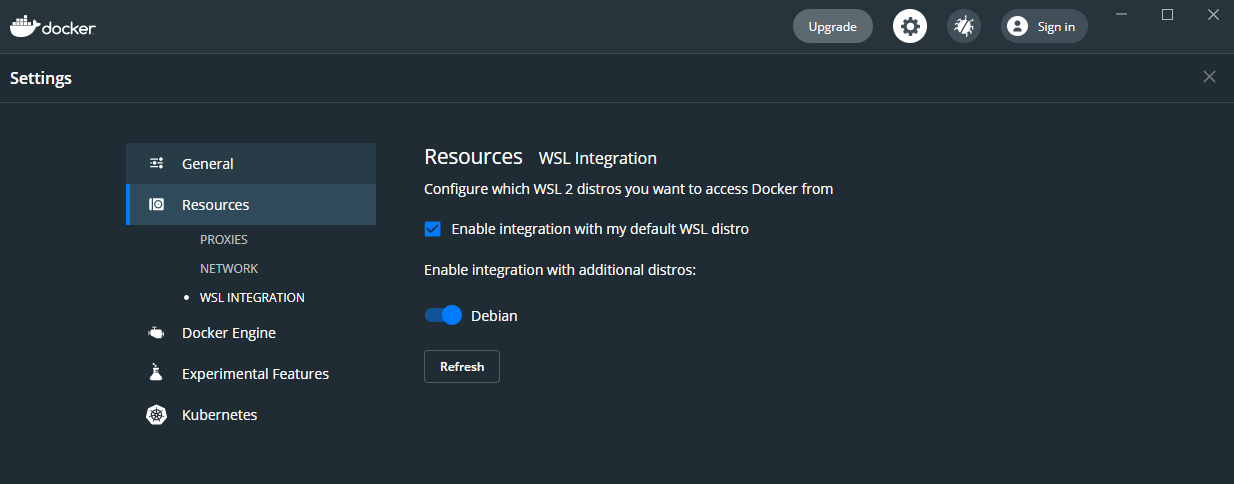
\includegraphics[width=1\linewidth]{webinterface/docker.png}
  \caption{Docker WSL Integration}
\end{figure}

Somit ist die Lokale Entwicklungsumgebung mit WSL und Docker abgeschlossen, die
benötigte Software wird später automatisch durch Laravel Sail in einem Docker
Container installiert.

\begin{figure}[H]
  \centering
  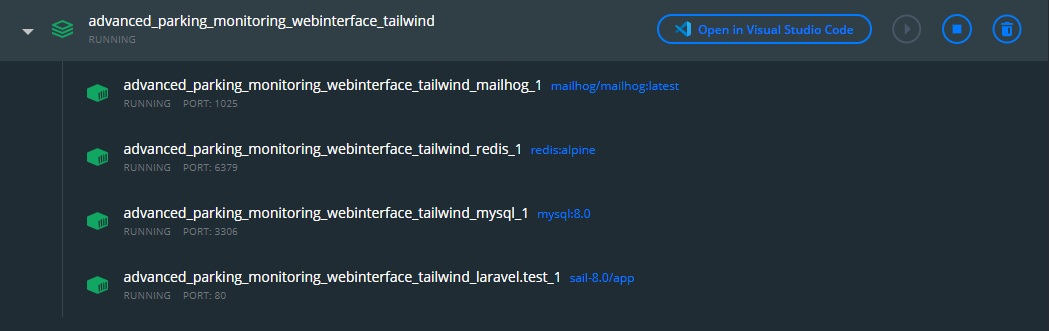
\includegraphics[width=1\linewidth]{webinterface/docker_container.png}
  \caption{Docker Container Steuerung}
\end{figure}

Es ist somit möglich die Services welche im Container in der Linux Distribution
laufen über die Docker Desktop Anwendung zu steuern.

\subsection{Production Server}
Der Production Server bzw. der Live Server ist der Server wo sich die Webanwendung
befindet und die Endbenutzer zugreifen, dieser Server wird auch einfach mit
Production abgekürzt. Der Production Server ist in diesem Fall ein Virtual
Private Server mit dem Betriebsystem Debian 10, welcher bei einem
Internet-Hosting Unternehmen mit Sitz in Deutschland gehostet wird.

\subsubsection{Benötigte Software}

Für den Live Server wird der sogenannte \glqq LAMP\grqq{} Stack verwendet. LAMP steht dabei
für die Software \textbf{L}inux, \textbf{A}pache, \textbf{M}ySQL und \textbf{P}HP.

\begin{itemize}
  \item \textbf{Apache Web Server} (\url{https://httpd.apache.org}) \\ HTTP Server
  \item \textbf{MariaDB} (\url{https://mariadb.org}) \\ Fork von MySQL
  \item \textbf{PHP} (\url{https://mariadb.org}) \\ Fork von MySQL
  \item \textbf{phpMyAdmin} (\url{https://www.phpmyadmin.net}) \\ Webinterface
  für MySQL
  \item \textbf{Composer} (\url{https://getcomposer.org}) \\ Paketmanager für PHP
  \item \textbf{Git} (\url{https://git-scm.com}) \\ Versionskontrolle
  Quelltext-Editor
\end{itemize}

\subsubsection{Installation des LAMP Stacks}
Bevor die Software Pakete installiert werden sollte die Linux Software/Update
Repository geupdatet werden.

\begin{lstlisting}[caption={Respositorys updaten}, captionpos=b]
  apt-get update && apt-get upgrade
\end{lstlisting}

\paragraph{Apache}\mbox{}\\

Nun kann der Apache Web Server installiert werden.

\begin{lstlisting}[caption={Apache installieren}, captionpos=b]
  apt install apache2
\end{lstlisting}

Die Installation kann nun leicht überprüft werden indem man im Browser die IP
bzw. die dazugehörige Domain öffnet, in diesem Fall:
(\url{http://dev.philipp-kraft.com}).

\begin{figure}[H]
  \centering
  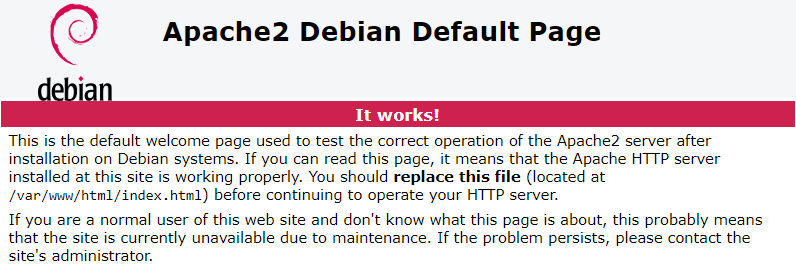
\includegraphics[width=1\linewidth]{webinterface/apache2_installation.png}
  \caption{Docker Container Steuerung}
\end{figure}

Erscheint die Debian Default Page ist Apache korrekt installiert.

\paragraph{PHP}\mbox{}\\
Neben PHP werden auch einige PHP Extensions benötigt.
\begin{lstlisting}[caption={PHP installieren}, captionpos=b]
  apt install wget php php-cgi php-mysqli php-pear php-mbstring
  php-gettext libapache2-mod-php php-common php-phpseclib php-mysql
\end{lstlisting}

Die Installation kann einfach mit dem Befehl \textbf{php -v} überprüft werden.

\paragraph{MariaDB}\mbox{}\\

\begin{lstlisting}[caption={MariadB installieren}, captionpos=b]
  apt install mariadb-server
\end{lstlisting}

Nun muss MariaDB noch konfiguriert werden.

\begin{lstlisting}[caption={MariaDB Secure Installation}, captionpos=b]
  mysql_secure_installation
\end{lstlisting}

Dabei wird dem root MySQL User ein Passwort gesetzt, Anonyme Benutzer gelöscht
und es werden Test Datenbanken gelöscht.

Nun wird ein neuer Benutzer mit root Berechtigungen erstellt.

\begin{lstlisting}[caption={MariaDB Secure Installation}, captionpos=b]
  mysql
  GRANT ALL ON *.* TO 'admin'@'localhost' IDENTIFIED 
  BY 'password' WITH GRANT OPTION;
  flush privileges;
  exit
\end{lstlisting}

\paragraph{phpMyAdmin}\mbox{}\\

Die aktuelle Version von phpMyAdmin kann von
(\url{https://www.phpmyadmin.net/downloads}) bezogen werden und mit dem
\textbf{wget} Befehl heruntergeladen werden.

\begin{lstlisting}[caption={phpMyAdmin Download}, captionpos=b]
  wget https://files.phpmyadmin.net/phpMyAdmin/5.0.4
  /phpMyAdmin-5.0.4-all-languages.tar.gz
\end{lstlisting}

Anschließend muss das Archiv entpackt werden.

\begin{lstlisting}[caption={phpMyAdmin Entpacken}, captionpos=b]
  tar xvf phpMyAdmin-5.0.4-all-languages.tar.gz
\end{lstlisting}

Als nächstes muss das entpackte Archiv in einen anderen Pfad verschoben werden
und zusätzlich müssen einige Rechte und Verzeichnisse angepasst werden.

\begin{lstlisting}[caption={phpMyAdmin Rechte und Verzeichnisse}, captionpos=b]
  mv phpMyAdmin-5.0.4-all-languages /usr/share/phpmyadmin
  mkdir -p /var/lib/phpmyadmin/tmp
  chown -R www-data:www-data /var/lib/phpmyadmin
  mkdir /etc/phpmyadmin/
\end{lstlisting}

Nun muss eine Konfigurations Datei erstellt werden und dort muss ein Blowfish
Secret\footnote{32 Zeichen String für Cookie-Authentifizierung} angegeben werden und den Pfad für ein Temporäres Verzeichnis.

\begin{lstlisting}[caption={phpMyAdmin Konfigurationsdatei erstellen}, captionpos=b]
  cp /usr/share/phpmyadmin/config.sample.inc.php  
  /usr/share/phpmyadmin/config.inc.php
\end{lstlisting}

und am Ende dieser Datei kann die zwei Zeilen eingefügt werden.

\begin{lstlisting}[caption={phpMyAdmin Blowfish Secret und TempDir}, captionpos=b]
  $cfg['blowfish_secret'] = 'H2OxcGXxflSd8JwrwVlh6KW6s2rER63i'; 
  $cfg['TempDir'] = '/var/lib/phpmyadmin/tmp';
\end{lstlisting}

Zuletzt muss der Apache Web Server konfiguriert werden.

Im Verzeichnis \textbf{/etc/apache2/sites-available} muss eine neue
Konfiguration angelegt werden \textbf{phpmyadmin.conf}. Diese Konfiguration
ermöglicht es, dass das Webinterface von phpMyAdmin über den Port 9000 (\url{http://dev.philipp-kraft.com:9000})
erreichbar ist und nicht wie Standardmäßig vorgesehen über das Verzeichnis
/phpmyadmin (\url{http://dev.philipp-kraft.com/phpmyadmin}), dies bietet einen Sicherheitsvorteil.

\begin{lstlisting}[caption={phpmyadmin.conf}, captionpos=b]
  Listen 9000

  <VirtualHost *:9000>
          ServerName localhost
  
          <Directory /usr/share/phpmyadmin>
                  AllowOverride None
                  Require all granted
          </Directory>
  
          DocumentRoot /usr/share/phpmyadmin
  
          ErrorLog ${APACHE_LOG_DIR}/phpmyadmin.error.log
          CustomLog ${APACHE_LOG_DIR}/phpmyadmin.access.log combined
  </VirtualHost>
\end{lstlisting}

Nun kann diese Virtual Host Konfigurations Datei aktiviert werden und danach
muss der Apache Web Server neu gestartet werden.

\begin{lstlisting}[caption={Virtual Host aktivieren}, captionpos=b]
  sudo a2ensite phpmyadmin
  sudo systemctl restart apache2
\end{lstlisting}